\chapter{Counting Feature Theory}
\label{chapterlabel4}

\section{Introduction to Counting Feature}

RTB has dramatically transformed the display advertising industry in the last a few years \cite{yuan2013real}. Similar to stock exchanges, RTB uses algorithms to transact advertisement placements automatically for each impression real-timely. Based on context information, user history and advertisement data, the advertisements are able to be targeted to specific users thus increasing the effectiveness of display advertising as well as saving cost for advertisers. Similar to the trend that trading is transformed form paper-based to automation in financial sector, the programmatic RTB has transformed the display advertising market subversively since 2010, started in USA. Figure \ref{fig:rtbmarket} presents the huge global opportunities in RTB, the spent money will increase by 135\% from 2012 to 2017, and RTB advertisements will increase by 456\%, an annual growth rate of  40\% in the RTB advertising industry can be expected\cite{rtb2015}.

\begin{figure}[h]
\centering
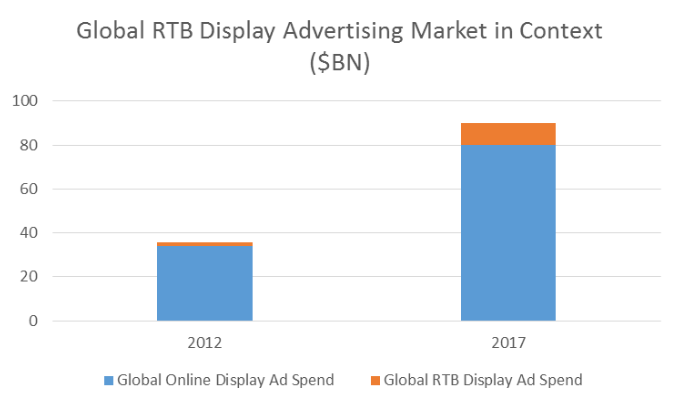
\includegraphics[width=\columnwidth]{rtbmarket.png}
\caption{Global RTB Display Advertising Market in Context}
\label{fig:rtbmarket}
\end{figure}

The core of \textit{computational advertising} is to find the \textit{optimal match} between \textit{advertisement} and \textit{users}, in some certain context \cite{balakrishnan2014real}. For the advertisers, a major concern is that whether their investments in online advertisement, like other business investments, can be paid back, namely the \textit{Return of Investment} (ROI). To specify, the profit can be represented as:\
\begin{equation}
profit = PV * CTR * ACP
\end{equation}

which is the realization formulation for sponsored search and RTB, \textit{PV} means \textit{Page View}, representing the volumes of retrieved ads, this is the upper bound of cash realization for advertising company, decided by the user experience of the recommended advertisements. \textit{CTR} means \textit{Click Through Rate}, it shows the average number of clicks for each advertisement impression, measuring the average click contribution for a single advertisement. Specifically, \textit{CTR} demonstrates the probability that one advertisement can be clicked, showing the accuracy of pushed advertisement to the audience. \textit{ACP} means \textit{Average Click Price}, which can be obtained by \(Total Cost / Total Clicks\). It is not surprising that PV, which is decide by the market share of the company and user experience, as well as ACP, which is decided by the company's strategy, are always fixed, therefore, in order to increase the ROI, predicting the CTR will be the crucial technology for advertisement and search engine companies, we can say that the CTR prediction is one of the most important part of the realization system of a company, which can be calculated by :

\begin{equation}
CTR = \frac{Clicks}{Impression} \times 100\%
\end{equation}

The key actors for CTR prediction problem can be shown in Figure \ref{fig:ctr}.

\begin{figure}[h]
\centering
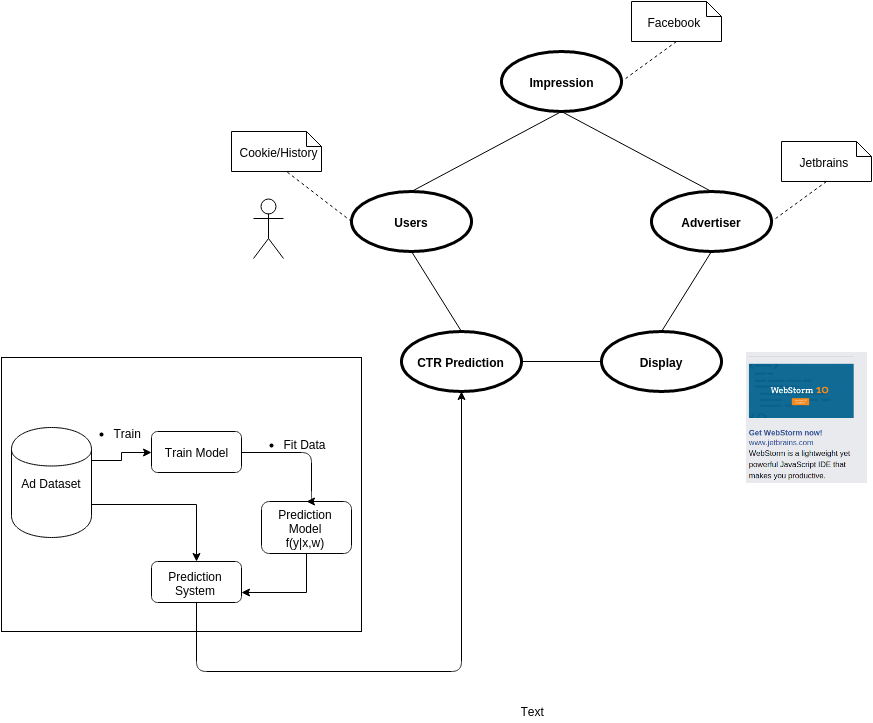
\includegraphics[width=\columnwidth]{ctr1.png}
\caption{CTR prediction Problem}
\label{fig:ctr}
\end{figure}

The challenges of the CTR prediction problem are multiple. Firstly, as we have entered the age of big data, hundreds of billions advertisements are presented every day \cite{lohr2012age}, many companies have already started the research on large-scale CTR prediction system, such as Google \cite{mcmahan2013ad}, Microsoft \cite{graepel2010web}, Baidu \cite{liu2012enlister} and Facebook \cite{he2014practical}. The problems they want to solve are similar to the challenges for big data, namely the \textit{3V} problem
\begin{itemize}
  \item Volume : With the exponential growth in the data storage for online advertisement, everyday billions of advertisements will be presented with more than a billion feature, unbalanced categories and huge data noise
  \item Velocity : The Ad data evolves a lot every second and the user behaviors change dramatically. CTR changes with time going, there are always new campaigns arising and old campaigns will expire.
  \item Variety : Advertisement data are from multiple sources, features are distinct for different campaigns, features are high dimensional and follow non-linear relations.
\end{itemize}
Therefore, the advanced online RTB advertising system must be able to handle the \textit{ZB-level, real-time} and \textit{high complexity} ad data. Models have to be trained and updated frequently and the strategies must be updated accordingly. 
The normal CTR prediction process can be represented as shown in Figure \ref{fig:system}

\begin{figure}[h]
\centering

\includegraphics[width=\columnwidth]{system.png}
\caption{Machine Learning Process of CTR Prediction}
\label{fig:system}
\end{figure}

Currently, most of the researches are based on how to build a better model and algorithms, however, as said in \cite{facebook2015}, in terms of the efforts of improving the performance of ML application, the significance of the three core factors are \(Data > Features > Algorithms\). The quality of data itself and the generated features decide the upper bound of the performance of CTR prediction problem, a better algorithm and model can only help reach this upper bound as near as possible. So in this paper I will refocus on the \textit{Feature Extraction}, or \textit{Feature Engineering} which are rarely discussed but only in a few literature and blogs, such as \cite{featureengineering}, and \cite{featureengineeringmeituan}. Based on existing unstructured and complex advertisements, better generated features will help reduce the complexity of model training and relieve the \textit{cold start} problem. The new features should have the following characters:
\begin{itemize}
  \item Low Dimensionality : With the explosion of data volume, the number features will grow extremely, without feature engineering, the feature numbers will follow a linear relation with the impression number, as \(O(n)\), \(n\) is the number of impressions in the advertisement dataset. Since for giant companies, like Google or Facebook, each day more than 100 billion impressions of ad data will be generated and distributed storing on thousands machines, we can imagine the astronomical number of features which will be trained and stored, currently, one-hot features are commonly used to generate discrete binary features, for example, imagine a company owns three types of features, which are \textit{User-related},\textit{Publisher-related} and \textit{Advertiser-related}, in each type there are 10 different categories, such as \textit{region},\textit{publisher network}, \textit{advertiser network},etc. So in total there are 30 categories for each impression. For a campaign, there are 1,000,000 impressions, since the number of features equals to the number of unique items in this dataset, so according to the situation from Adform and iPinYou dataset, 5,000,000 will be a possible number of features, an impression vector will look like:
\begin{equation}
 \Big[\underbrace{[0,0,1....0,0,0]}_\textrm{Advertiser Network} + \underbrace{[0,1,0,0,0....0,0,0]}_\textrm{Publisher Network}.... \underbrace{[0,1,0,0....0,0,0]}_\textrm{Region}]
\end{equation}
Therefore, the binary one-hot feature is high dimensional and extremely sparse, and with the new come-in advertisement data, such as the ones from new campaigns, the number of features will also increase accordingly. So it is more efficient to replace the redundant and cumbersome binary feature with the feature with lower and fixed dimensions.

    \item Scalability : A huge drawback of binary feature is its lack of scalability. Imagine for Adform the old campaigns are form UK, and the CTR prediction model is trained based on the unique \textit{British Feature}, however, when a new campaign from Netherlands comes in, the overlap between the feature sets of UK old campaigns and Dutch new campaign will be small, at least the category \textit{Region} will be totally different, so the model can be only used for old campaigns and will be abandoned for new ones. Some researches have studied on how to build the model on new campaigns, but no generalized method has been proposed which is able to be used for all kinds of campaigns.
    
    \item Feature Explainability : Some companies and researchers have turned to deep learning and try to apply this magical method in the field of CTR prediction, such as the studies from \cite{deeplearning} and \cite{wang2014collaborative}, indeed, many companies now run distributed classification system for CTR prediction problems, the data training process has to be finished on Amazon EC2, but on the one hand, the method used well on one computer dose not mean that it will run perfect on distributed system, on the other hand, if deep learning is used, maybe it can improve the performance somewhat, however, firstly, it is hard to implement, secondly, the learned parameters and weights are hard to be explained , the parameters of this \textit{Black Box} cannot be interpreted with physical meanings.  
    
\end{itemize}

In order to meet the above three requirements, we propose the concept of \textit{Counting Feature}, which is totally different from the traditional \textit{Binary Feature} which is converted from categorical variables to one-hot vectors, thus sparse and mostly zeros. The counting feature essentially is a kind of \textit{statistical feature}, the one we expound is composed of \textit{Frequency Feature} and \textit{Average CTR Feature} as we discussed above. Therefore, for each categorical field in the dataset two features will be generated. For example, if we have a dataset with 3 fields, \textit{Region}, \textit{Hour}, and \textit{Cookie ID}, the the binary feature will be like: 

\begin{equation}
 \Big[\underbrace{[0,0,1....0,0,0]}_\textrm{Region} + \underbrace{[0,1,0,0,0....0,0,0]}_\textrm{Hour}.... \underbrace{[0,1,0,0....0,0,0]}_\textrm{Cookie ID}]
\end{equation}

and counting feature will be like:

\begin{equation}
 \Big[\underbrace{[0.0034,0.0001]}_\textrm{Region} + \underbrace{[0.0345,0.0002]}_\textrm{Hour}.... \underbrace{[0.0001,0]}_\textrm{Cookie ID}]
\end{equation}

Therefor counting feature can dramatically reduce the dimensionality of feature space, as shown in Figure ~\ref{fig:dimensionreduct}.

\begin{figure}[h]
\centering
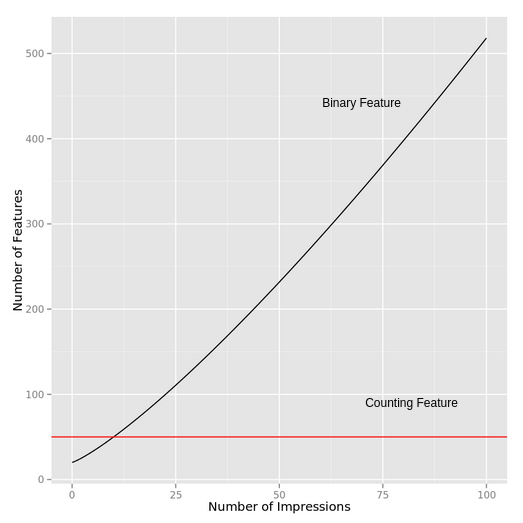
\includegraphics[scale=1.5]{dimensioncurse.png}
\caption{Dimensionality Reduction of Counting Feature}
\label{fig:dimensionreduct}
\end{figure}

Also counting feature is easy to be stretched. As we present in the \textit{Dataset Introduction} part in Chapter 5, the log data format will be the same for a certain company. The impressions is stored in the database on row-per-record basis and each field is represented in one column. Therefore, since the number of features are the same among all advertising campaigns with corresponding relations, the weights of the features learned from one campaign are feasible to be used for others, unlike binary features whose features will be unique for one campaign and cannot be scalable. 

At last, it is obvious that the parameters of the model trained using counting feature can be easily explained, for example, if the weight for the \textit{Frequency Feature} of the field \textit{Hour} is higher than the others, it means that the time when people browse the webpages play a crucial role to affect the human behavior to click on the advertisements.

One thing needed to point out here is that there are already many researches on \textit{Dimensionality Reduction}, such as \cite{burges2009dimension}, most of them are from the field of Natural Language Processing (NLP), a popular method will be Principle Component Analysis (PCA). As the method in \cite{fruergaard2013dimensionality} and \cite{dimensionreduct}, the goal of PCA is, given a \(N\) dimension space \(\mathbf{x}=(x_1,\ldots,x_n)^T\), to find a direction, namely a \(N\) dimension vector \(\mathbf{w}=(w_1,\ldots,w_n)^T\) to make sure the the linear combination \(\sum_{i=1}^nw_ix_i=\mathbf{w}^T\mathbf{x}\) can be obtained with the minimal reconstruction error or maximal characteristic. But PCA seems not applicable for the problem of CTR predtion, because:

\begin{itemize}
  \item In the PCA algorithm, firstly we need to create \(N \times d\) data matrix, in which one row vector \(x_n\) represents one data point, after subtracting the mean of \(x\) from the matrix, we need to calculate the covariance matrix of \(x\) and find eigenvectors and eigenvalues, which will take time of \(O(N*D^2)\) and memory of \(O(2*D^2)\), using SVD with another time complexity of \(O(D^3)\). Therefore it is obvious that PCA algorithm is computational intensive, especially when the number of impressions is at the level of 10 million with more than 10 million features, it is impossible to solve such a huge matrix locally. 
  \item From the view of NLP, the principle, or topics of each impression binary vector will be obtained using PCA algorithm, but unlike NLP, in the field of online advertising, we can just regard each topic as one field in the dataset, and use GBRT or other algorithms to obtain the combination of topics easily, there is no need to use PCA method.
  \item The most important thing is PCA algorithms finds the principle components by coordinate rotation, if the input feature space is not Gaussian Distribution, then the eigenvalues and eigenvectors cannot represent the characteristic of the feature distribution. It is not surprising that the sparse binary feature space does not follow a normal distribution, so PCA is not applicable here. 
\end{itemize}

Therefore, we believe counting feature is the only feature space to satisfy the above three requirements and we will discuss on its properties and performance in the rest of the paper. 


\section{Relation Between Counting Feature and Binary Feature}
In this section we will present the deduction of the relation between \textit{Counting Feature} and \textit{Binary Feature} in the context of \textit{Linear Regression Model}, in the field of online advertising, each data porint is \(Impression = \{ x_i,y_i \}_{1 \leq i \leq N}\)  where each \(x_i  \in \mathbb{R}^n\) and \(y_i \in \mathbb{R}\), and \(N\) is the number of impressions in the dataset, \(x\) is the feature space and \(y\) is the click label. Assuming that the click label follows the basic linear relation with feature space, as follows:
\begin{equation}
y_i =w_0 +\sum_j w_j x_{ij} =w_0 +w^T x_i 
\end{equation}
By redefining \(x_i = (1,x_i)\) and combining \(w_0\) and \(w_i‘s\) into a single weights vector we can get 
\begin{equation}
y_ i = w^T x_i 
\end{equation}

According to \cite{prince2012computer} and use \textit{Maximum Likelihood Estimation} method, the click label \(y_i\) can be assumed to have Gaussian noise error, \begin{equation}
y_i = w^T x_i + \epsilon 
\end{equation}
where \(\epsilon \sim N(0,\sigma^2)\).
Then the likelihood can be obtained by :
\begin{equation}
\mathcal{L}(D | w, \sigma) = (2 \pi \sigma^2)^{-n/2} \prod_{i=1}^{n} exp \left[ \frac{-(y_i - \hat{y}_i)^2}{2\sigma^2} \right] 
\end{equation}
and 
\begin{equation}
w_{MLE} = argmin_w \sum_i  (y_i - w^T x_i)^2 
\end{equation}
At last we can obtain that 
\begin{equation}\label{eq:w}
\hat{W} = (X^T X)^{-1} X^T Y 
\end{equation}
in which  \(X = (x_1, x_2, \ldots, x_N)^T\), \(Y = (y_1, y_2, \ldots, y_N)^T\) and \(W = (w_0, w_1, w_2, \ldots, w_N)^T\)

In the rest of this section, we will demonstrate how to transform the weight space of binary feature to that of \textit{Frequency Feature} and \textit{Average CTR Feature} respectively, the notation used in the math equations in the rest of the section is shown in Table \ref{tab:notation-des}
\begin{table}[h]
\center
\vspace{-5pt}
\caption{Notations and descriptions.}
\label{tab:notation-des}
\small
\begin{tabular}{rl}
Notation & Description\\
\hline
\\ [-2.0ex]
$\bs{x_{\text{b}(N\times D)}}$ & The one-hot binary feature space.\\
$\bs{x_{\text{c}(N\times D)}}$ & The continuous counting feature space.\\
$\bs{y_{(1\times N)}}$ & The click result space\\
$w_{\text{b}(1\times D)}$ & The weights vector space of binary feature\\
$w_{\text{c}(1\times D)}$ & The weights vector space of counting feature\\
$T_{(M\times D)}$ & Transform Binary Feature to Counting Feature matrix\\
$A_{(N\times 1)}$ & Calculating frequency matrix which is an all-one vector $\vec{1 }$\\
$C_{(M\times D)}$ & Field  matrix which is a 0-1 matrix concatenated with \textsl{}{M} \\
& vectors \(V_{m,(m = 1...M)}\) and in each vector \(V_m\) only its \\
& corresponding positions in field \textsl{m} is filled with 1, \\
& with other positions 0. \\
$Diag$ & Transform the column vector into a diagonal matrix
\end{tabular}
\end{table}


\subsection{Frequency Feature}

The CTR predictino problem can be regarded as a classical classification problem in Machine Learning, we can use features of ads, terms, and advertisers to learn a model that accurately predicts the CTR for new ads. The training dataset contains a number of \textsl{N} instances, which are the records in datalog containing \textsl{M} fields of user, advertiser and publisher information, as well as their click label for each ad impression. The result of the impression, namely whether the user clicks on the ad will be represent by \textsl{y}. Since here the dependent variable is dichotomous, the liner regression can be used to prove the relation between model built by \(x_{\text{c}}\) representing the data instances encoded into \textsl{Counting Feature} and model built by \(x_{\text{b}}\) representing the data instances encoded into one-hot \textsl{Binary Feature}. The dimension of the \textit{frequency feature} and \textit{average CTR feature} is the number of fields \textsl{M} well the dimension of \(x_{\text{binary}}\) is represend by \textsl{D} for which \(D >> M\). The more detailed information about symbols are shown in Table 3.1.
\iffalse
\begin{itemize}
\item  Binary Features : \(x_{\text{binary}(N\times D)}\)
\item  Counting Feature : \(x_{\text{counting}(N\times D)}\)
\item  Clicking result : \(y_{(1\times N)}\)
\item  Weights vector of Binary Feature : \(w_{\text{binary}(1\times D)}\)
\item  Weights vector of Counting Feature: \(w_{\text{counting}(1\times M)}\)
\item  Transform Binary Feature to Counting Feature matrix : \(T_{(M\times D)}\)
\item  Calculating feaquency matrix : \(A_{(N\times 1)}\) which is an all-one vector 
$\vec{1 }$  
\item  Field  matrix : \(C_{(M\times D)}\) which is a 0-1 matrix concatenated with \textsl{}{M} vectors \(V_{m,(m = 1...M)}\) and in each vector \(V_m\) only its corresponding positions in field \textsl{m} is filled with 1, with other positions 0.
\item  Diag function : Transform the column vector into a diagonal matrix.\vspace{5mm} 

\end{itemize}
\fi
 It can be proven that 
\[ T = C\times Diag(x_{b}A) \]
The formation of \textsl{T} is 

$$
\begin{pmatrix} 
\vec{F_1} \\
\vec{F_2} \\
.\\
\vec{F_M}

\end{pmatrix}
$$

\noindent in which \($$\vec{F_m}$$ = $$\begin{pmatrix} 
$$\vec{0 }$$ , f_{m1}, f_{m2}, ...f_{mi}... , f_{mI} ,$$\vec{0 }$$ 
\end{pmatrix}$$\), and \(f_{mi}\) represents the occurrence of \(i_{th}\) binary feature in the field \textsl{m} in the whole dataset.\vspace{5mm}

\noindent Next, the relations between \(w_{\text{binary}}\) and \(w_{\text{counting}}\) are proven as follows. 

\begin{equation}
w_{\text{b}} \times x_{\text{b}}^T = y 
\end{equation}

\begin{equation}
(w_{\text{b}}^T \times w_{\text{b}}) \times x_{\text{b}}^T = w_{\text{b}}^T \times y 
\end{equation}

\begin{equation}
x_{\text{b}}^T = (w_{\text{b}}^T \times w_{\text{b}})^{-1} \times w_{\text{b}}^T \times y 
\end{equation}

Using SVD, we can derive that,

\begin{equation}
(w_{\text{b}}^T \times w_{\text{b}})^{-1} \times w_{\text{b}}^T = (w_{\text{b}})^{-1(left)}  
\end{equation}

So we can get that 
\begin{equation}
x_{\text{b}}^T =  (w_{\text{b}})^{-1(left)} \times y 
\end{equation}

We define
\begin{equation}
T = C \times Diag(x_{\text{b}}^T \times A)
\end{equation}


Multiply each size by \textsl{T}, we can get
 
\begin{equation}
T \times x_{\text{b}}^T =  T \times (w_{\text{b}})^{-1(left)} \times y 
\end{equation}

It can be proven that 
\begin{equation}
T \times x_{\text{b}}^T =  x_{\text{c}}
\end{equation}

So
\begin{equation}
x_{\text{c}} =  T \times (w_{\text{b}})^{-1(left)} \times y 
\end{equation}

Since \(T \times (w_{\text{b}})^{-1(left)}\) is a \(M \times 1\) matrix, so multiplying its transposition we can get a constant scalar, 
\begin{equation}
(T \times (w_{\text{b}})^{-1(left)})^T \times (T \times (w_{\text{b}})^{-1(left)}) = \lambda
\end{equation}

So, 
\begin{equation}
1/{\lambda} \times (T \times (w_{\text{b}})^{-1(left)})^T \times x_{\text{c}} =  y
\end{equation}

In conclusion, we can get
\begin{equation} \label{eq:12}
\begin{split}
w_{\text{c}} & =\ 1/{\lambda} \times (T \times (w_{\text{b}})^{-1(left)})^T \\
& = \ 1/{\lambda} \times (C \times Diag(x_{\text{b}}^T \times A) \times (w_{\text{b}})^{-1(left)})^T
\end{split}
\end{equation}

substitute \(W\) with \((X^T X)^{-1} X^T Y\), we can get:
\begin{equation} \label{eq:13}
\begin{split}
w_{\text{c}} & =\ 1/{\lambda} \times (T \times (w_{\text{b}})^{-1(left)})^T \\
& = \ 1/{\lambda} \times (C \times Diag(x_{\text{b}}^T \times A) \times ((x_{\text{b}}^T x_{\text{b}})^{-1} x_{\text{b}}^T y)^{-1(left)})^T
\end{split}
\end{equation}

\subsection{Average CTR feature}

\setlength{\parindent}{5ex}

In this section, the relation between  \(w_{\text{ctr}}\) and \(w_{\text{binary}}\) will be deduced, the steps are similar except for specific part of CTR calculating. 

Initially, we can get the similar deduction process, 
\begin{equation}
w_{\text{b}} \times x_{\text{b}}^T = y 
\end{equation}

\begin{equation}
(w_{\text{b}}^T \times w_{\text{b}}) \times x_{\text{b}}^T = w_{\text{b}}^T \times y 
\end{equation}

\begin{equation}
x_{\text{b}}^T = (w_{\text{b}}^T \times w_{\text{b}})^{-1} \times w_{\text{b}}^T \times y 
\end{equation}

\begin{equation}
(w_{\text{b}}^T \times w_{\text{b}})^{-1} \times w_{\text{b}}^T = (w_{\text{b}})^{-1(left)}  
\end{equation}

\begin{equation}
x_{\text{b}}^T =  (w_{\text{b}})^{-1(left)} \times y 
\end{equation}

However, then in order to count the number of \textsl{clicks} for each instance, we redefine the transformation matrix \textsl{T} as following, 

\begin{equation}
T_{\text{click}} = C \times Diag(x_{\text{b}}^T \times y)
\end{equation}



From section 1, we can know that, 
\begin{equation}
T_{\text{frequency}} = C \times Diag(x_{\text{b}}^T \times A)
\end{equation}

Since it is easy to know that,

\begin{equation}
(Diag(T_{\text{click}}) \times (1/T_{\text{frequency}} )^T =  T_{\text{ctr}}
\end{equation}

Similar to section 1, we can multiply \(T_{\text{ctr}}\) by both sides of equation (17)

\begin{equation}
T_{\text{ctr}} \times x_{\text{b}}^T =  T_{\text{ctr}} \times (w_{\text{b}})^{-1(left)} \times y 
\end{equation}

It can be proven that 

\begin{equation}
T_{\text{ctr}} \times x_{\text{b}}^T =  x_{\text{ctr}}
\end{equation}

So,

\begin{equation}
 x_{\text{ctr}} =  T_{\text{ctr}} \times (w_{\text{b}})^{-1(left)} \times y 
\end{equation}

It is similar to section 1 that \(T_{\text{ctr}} \times (w_{\text{binary}})^{-1(left)}\)is a \(M \times 1\) matrix, so we define, 
\begin{equation}
(T_{\text{ctr}} \times (w_{\text{b}})^{-1(left)})^T \times (T_{\text{ctr}} \times (w_{\text{b}})^{-1(left)}) = \lambda
\end{equation}

So, 
\begin{equation}
1/{\lambda} \times (T_{\text{ctr}} \times (w_{\text{b}})^{-1(left)})^T \times x_{\text{ctr}} =  y
\end{equation}

In conclusion, we can get
\begin{equation} 
\begin{split}
w_{\text{ctr}} & =\ 1/{\lambda} \times (T_{\text{ctr}} \times (w_{\text{b}})^{-1(left)})^T \\
& = \ 1/{\lambda} \times (Diag(T_{\text{click}}) \times (1/T_{\text{frequency}} )^T \\ 
& \times (w_{\text{b}})^{-1(left)})^T \\
& = \ 1/{\lambda} \times (Diag(C \times Diag(x_{\text{b}}^T \times y)) \\ 
& \times (1/ (C \times Diag(x_{\text{b}}^T \times A) )^T) \times (w_{\text{b}})^{-1(left)})^T
\end{split}
\end{equation}
and
\begin{equation} 
\begin{split}
w_{\text{ctr}} & =\ 1/{\lambda} \times (T_{\text{ctr}} \times (w_{\text{b}})^{-1(left)})^T \\
& = \ 1/{\lambda} \times (Diag(T_{\text{click}}) \times (1/T_{\text{frequency}} )^T \\ 
& \times (w_{\text{b}})^{-1(left)})^T \\
& = \ 1/{\lambda} \times (Diag(C \times Diag(x_{\text{b}}^T \times y)) \\ 
& \times (1/ (C \times Diag(x_{\text{b}}^T \times A) )^T) \times ((x_{\text{b}}^T x_{\text{b}})^{-1} x_{\text{b}}^T y)^{-1(left)})^T
\end{split}
\end{equation}

\subsection{Non-linearity of Counting Feature}
From the above deduction, we can draw the conclusions that
\begin{itemize}
\item The transformation matrix can help transform the high-dimension binary feature space into low-dimension counting feature space, which is a non-linear transformation.
\imte The weight space of binary feature model can be transformed into that of counting feature model in a non-linear way.
\end{itemize}
In the following of the paper, we will use \textit{logistic regression} which is a popular discriminative classifier to directly learn \(P(Y|X)\) and model the binary class boundary for \textit{Binary Feature}, as follows:
\begin{equation}
P(Y = 1| X) = \frac{exp(w_{0} + \sum_{i = 1}^{n} w_{i}x_{i})}{1 + \exp(w_{0} + \sum_{i = 1}^{n} w_{i}x_{i})}  
\end{equation}
and 
\begin{equation}
P(Y = 0| X) = \frac{1}{1 + \exp(w_{0} + \sum_{i = 1}^{n} w_{i}x_{i})}  
\end{equation}
The precondition of using logistic regression is that the dependant features and the target (click) follow the linear regression, since we already know that the \textit{counting feature} is a non-linear transformation of \textit{binary feature}, we can define the non-linear formulation of logistic regression as follows:
\begin{equation}
Pr(w_{\text{i}}|x_{\text{i}}) = Bern_{w_{\text{i}}}[sig(a_{\text{i}})]
\end{equation} \cite{prince2012computer}

in which \(sig(a_{\text{i}})\) is the sigmoid function and the activation \(a_{\text{i}}\) is given by,

\begin{equation}
a_{\text{i}} = \Phi^T f(x_{\text{i}})
\end{equation}

The function and \(f(x)\) is the nonlinear transformation of the space \(x\), \(f(x_{\text{i}})\) can be represented as \(T x_{\text{b}}^T \) in terms of \textit{Frequency Feature} (Average CTR Feature has a similar relation), that is:
\begin{equation}
f(x_j) = \sum_{i=1}^{D}T_{ji} x_\text{b}_i  
\end{equation}
in which \(j\) is the \(j_th\) field of the dataset and \(i\) is the \(i_th\) dimension of binary feature. 

In our case of frequency feature and average CTR feature, the weights space should be derived as \(\Phi^T \) using incremental fitting and boosting model. 

%So we successfully transform the linear logistic regression on \(N\) dimension to the incremental fitting and boosting problem, we will do some experiment to prove the equivalence of them.

\begin{figure}[h]
\centering
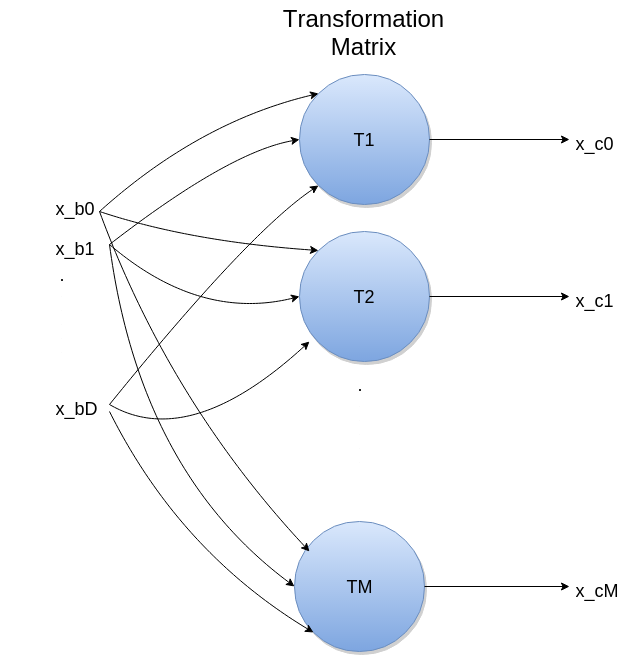
\includegraphics[scale = 1.5]{countingfeature.png}
\caption{Binary Feature to Counting Feature}
\label{fig:counting}
\end{figure}
In summary, we can see \textit{counting feature} as a nonlinear transformation from \textit{binary feature} from the same dataset, which can be seen as a statistical representation of binary feature, compressing the information of the whole dataset. Counting feature can reduce the high dimension of binary feature to lower dimensions, namely from millions of dimensions to less than 1 hundred. The cost of this reduction is assuming that binary feature follows a linear model to the label, such a space transformation will lead to the non-linearity of the counting feature. So we have to use non-linear regression model, such as Gradient Boosting Decision Decision (GBDT) to solve this problem. Using the method in \cite{he2014practical}, one way to do so is to transform the input space so that the non-linearity is eliminated and a linear feature space can be obtained, this can be done by GBDT, and according to \cite{cover1965geometrical}:

\textit{"A complex pattern-classification problem, cast in a high-dimensional space nonlinearly, is more likely to be linearly separable than in a low-dimensional space, provided that the space is not densely populated."}

So the counting feature can be trained into the model when following a non-linear regression model to eliminate the non-linearity meanwhile obtain the comparable performance in terms of CTR prediction with binary feature.

In Chapter 5.2, we will show the performance comparison of binary feature and counting feature in the context of real world online advertising dataset from Adform using both Logistic Regression Model and GBDT model. 
The logistic regression model is:
\begin{equation}
CTR = P(Y|X,w) = \frac{1}{1 + \exp(-a)}  
\end{equation}
In which \(a = \phi^T x\)

Using the training dataset \((x_i,y_i)\), and using \(L_\text{1}\) regularization, we can get the loss function as:
\begin{equation}  \label{eq:object}
min_w \sum_{i}^{N} [y_i In(1+\exp {-w^T x_i}) + (1-y_i) In(1+\exp {w^T x_i})] + c||w||_1, ||w|| = \sum_j=1^D |w_j|
\end{equation}

And we will use Newton Method to solve the problem, the gradient ascent computes the most optimal parameters by updating in the direction of gradient iteratively as 
\begin{equation}
w_{i} \rightarrow w_{i} + \alpha \frac{\partial l(w)}{\partial w_{i}}  
\end{equation}
where 
\begin{equation}
\frac{\partial l(w)}{\partial w_{i}} = \sum_{t} X^{t}_{i}(Y^{t} - \hat{P}(Y^{t} = 1|X^{t}, w))  
\end{equation}

As for GBDT algorithm, referring to the method in \cite{boostedtree}, we will use the idea of \textit{boosted trees} to realize the non-linear logistic CTR prediction model. The objective function of GBDT can be regarded as the same as \ref{eq:object}, the tree ensemble model is used here which is the \textit{classification and regression trees} (CART). For each classification tree we can obtain a score for the prediction task, the sum up of the scores from individual tree will lead to the final score of prediction. The model can be fomulated as:
\begin{equation}
y_i = \sum_{k=1}^K f_k(x_i), f_k \in F
\end{equation}
where \(K\) is the number of trees, and \(f\) is a function in the functional space of all possible CARTs. Using the method of \textit{Additive Training} the objective method can be solved and the parameters of the trees can be obtained. The details of the GBDT method can be referred in \cite{boostedtree} and \cite{he2014practical}.

The comparison results show that the performance of counting feature using non-linear regression model (GBDT) is comparable to that of binary feature using linear regression model (Logistic regression model), using Area under the curve (AUC) as the criteria, which proves the correctness and retionality of counting feature.

\section{Counting Feature Generalization}
In this part, we will briefly discuss on the generalization of counting feature, to prepare for the next chapter. Our assumption is that counting feature has a better property of generalization than binary feature, we have the following backup which is considered in terms of weight space of the CTR prediction models.
We will compare the weight space of binary and counting feature, from \ref{eq:12} we can get the following equation:
\begin{equation} \label{eq:28}
\begin{split}
w_{\text{counting}} & =\ 1/{\lambda} \times (C \times Diag(x_{\text{binary}}^T \times A) \times (w_{\text{binary}})^{-1(left)})^T \\
& = \ 1/{\lambda} \times (C \times Diag(x_{\text{binary}}^T \times A) \times ((w_{\text{binary}}^T \times w_{\text{binary}})^{-1} \\
& \times w_{\text{binary}}^T )^T
\end{split}
\end{equation} 

It is obvious that the dimension of counting feature is much less than binary feature. Imagine we have two campaigns from each we can obtain the weight space using logistic regression model, which are \(w_1\) and \(w_2\). Mathematically, we know that in the space the included angle \(\theta\) of two vectors in \(n\) dimension follow the probability density function of 

\begin{equation}
p(\theta)=\frac{\Gamma(\frac{n}{2})}{\Gamma(\frac{n-1}{2})}
\frac{\sin^{n-2}(\theta)}{\sqrt\pi}
\end{equation}

Therefore in a high dimension the two vectors will be almost vertical to each other, which means the weight space of binary features for two campaigns will be uncorrelated to each other

In Figure \ref{fig:three graphs}, using the top 10 campaigns from Adform dataset which is introduced in detail in Chapter 5, we do the experiment as follows,
\begin{enumerate}
\item we train the CTR prediction model using logistic regression model for each campaign in terms of counting feature and binary feature, to obtain \([w_{b1},w_{b2},...w_{b10}]\), and \([w_{c1},w_{c2},...w_{c10}]\)
\item Then for the 10 binary weight spaces and counting weight spaces, we calculate the cos similarity, correlation, and euclidean distance for each pair of the weights space
\end{enumerate}
 
The result is shown in Figure \ref{fig:three graphs} from which we can see the weight space of counting feature are much more similar to each other than that among binary features.
\begin{figure}[h]
    \centering
    \begin{subfigure}{0.3\textwidth}
        \includegraphics[width=\textwidth]{cos}
        \caption{Cos Similarity Comparison Between Pairwise of Binary Feature and Counting Feature}
        \label{fig:cos}
    \end{subfigure}
    \hfill
    \begin{subfigure}{0.3\textwidth}
        \includegraphics[width=\textwidth]{correlation}
        \caption{Correlation Similarity Comparison Between Pairwise of Binary Feature and Counting Feature}
        \label{fig:correlation}
    \end{subfigure}
    \hfill
    \begin{subfigure}{0.3\textwidth}
        \includegraphics[width=\textwidth]{euclidean}
        \caption{Euclidean Distance Comparison Between Pairwise of Binary Feature and Counting Feature}
        \label{fig:euclidean}
    \end{subfigure}
    \caption{Comparison of Binary and Counting Feature Model Weights Space}
    \label{fig:three graphs}
\end{figure}
%Now the experiment is done in which the placement id is counted and when the clicks in one palcement id's corresponding is higher than 200, the instances will be remained, and the overlap of placement id in the train dataset and test dataset will be filtered out. Then for the training dataset all the campains in the test dataset are new. Many experiments are done now but result is confused. Generally the result is as follows: 

From Figure \ref{fig:three graphs} it shows the similarities among weight spaces of counting feature are significantly higher than that of binary feature, and weight spaces of binary feature are hardly related.  Therefore, we can say that since the counting values are continuous ranging from 0 to 1, the variability of data distribution among different campaigns are largely transformed from weight space to feature space for counting feature. Even though directly using the weight space trained from old campaign to new campaign will lead to poor performance initially for both counting feature and binary feature, with the income new data containing the information of distribution from new campaign, we are able to update the values of counting feature to force the model trained from the old campaign to be \textit{alike} the new campaign, however for binary feature the variability of the model is taken by the weight space since there are only 0 and 1 for the binary feature value, so it is not possible to transform the statistical information from new campaign to the old model. 

So it is reasonable to presume that counting feature can be used to alleviate the cold start problem.

\iffalse
I am trying to figure out the reason why binary feature performs well in cold start problem and it seems biased dataset is a cause and I try to split the model into generic and specific parts and overcome the bias.
\subsection{Model Similarity Analysis}
At first, we will start from the easier one, the frequency feature. Let's assume that we have two datasets, dataset \(Dataset_{\text{1}}\) and \(Dataset_{\text{2}}\), for each dataset we can get \(w_{\text{counting}}\) and \(w_{\text{binary}}\) respectively. Let's abbreviate them as \(w_{\text{c1}}\) and \(w_{\text{b1}}\) as well as \(w_{\text{c2}}\) and \(w_{\text{b2}}\). 

From \ref{eq:12} we can get the following equation:
\begin{equation} \label{eq:28}
\begin{split}
w_{\text{counting}} & =\ 1/{\lambda} \times (C \times Diag(x_{\text{binary}}^T \times A) \times (w_{\text{binary}})^{-1(left)})^T \\
& = \ 1/{\lambda} \times (C \times Diag(x_{\text{binary}}^T \times A) \times ((w_{\text{binary}}^T \times w_{\text{binary}})^{-1} \\
& \times w_{\text{binary}}^T )^T
\end{split}
\end{equation}

We will make use of cos similarity, which is used to measure the distance between two vectors to measure the similarity of two \(w_{\text{counting}}\) from \(Dataset_{\text{1}}\) and \(Dataset_{\text{2}}\). The formation of similarity can be shown as follows:

\begin{equation} \label{29} 
\begin{split}
Similarity & = \cos(\Theta) = \frac{w_{\text{c1}} \times w_{\text{c2}}^T} {||w_{\text{c1}}|| \times ||w_{\text{c2}}|| }
\end{split}
\end{equation}

Substitute \(w_{\text{c1}}\) with \ref{eq:12} and represent \(Diag(x_{\text{binary}}^T \times A)\) using \(Diag(f)\) since this diagonal entries \(d(i,i) \) shows the frequency of feature \(i\), we can get the following equation:


\begin{equation} \label{30} 
\begin{split}
\frac{w_{\text{c1}} \times w_{\text{c2}}^T} {||w_{\text{c1}}|| \times ||w_{\text{c2}}|| } & =  \frac{w_{\text{c1}} \times w_{\text{c2}}^T} {\sqrt{w_{\text{c1}} \times w_{\text{c1}}^T} \times \sqrt{w_{\text{c1}} \times w_{\text{c2}}^T} }
\end{split}
\end{equation}

To simply, at first we will deduct the following equation:

\begin{equation} \label{31} 
\begin{split}
w_{\text{ci}} \times w_{\text{cj}}^T & = \frac{1}{{\lambda}_{i}{\lambda}_{j} } \times (w_{\text{bi}} \times Trans_{i}) \times (w_{\text{bj}} \times Trans_{j})^T \\
& subject : (i.j = 1 \cup 2)
\end{split}
\end{equation}

\fi
%In which \(Trans\) is a Transformation Matrix, 
%\begin{equation} \label{31} 
%\begin{split}
%Trans = ((w_{\text{binary}}^T \times w_{\text{binary}})^{-1})^T \times (Diag(f))^T \times C^T  
%\end{split}
%\end{equation}

%Then, we will focus on the transformation matrix. 

%Since \(((w_{\text{binary}}^T \times w_{\text{binary}})^{-1})^T\) is a symmetric matrix, so it equals to its own transposition. 


